\documentclass[11pt,a4paper]{article}
\usepackage[T1]{fontenc}
\usepackage[utf8]{inputenc}
\usepackage{lmodern}
\usepackage[margin=1in]{geometry}
\usepackage{amsmath,amssymb,amsthm,mathtools}
\usepackage{booktabs,tabularx,array}
\usepackage{enumitem}
\usepackage{xcolor}
\usepackage{microtype}
\usepackage{pgfplots}
\pgfplotsset{compat=1.18}
\usetikzlibrary{patterns,decorations.pathreplacing,calc}
\usepackage[numbers,sort&compress]{natbib}
\usepackage[colorlinks=true,linkcolor=blue!50!black,citecolor=blue!50!black,urlcolor=blue!50!black]{hyperref}
\usepackage[capitalise,noabbrev]{cleveref}

\theoremstyle{plain}
\newtheorem{theorem}{Theorem}
\newtheorem{proposition}{Proposition}
\newtheorem{lemma}{Lemma}
\newtheorem{corollary}{Corollary}
\theoremstyle{definition}
\newtheorem{definition}{Definition}
\newtheorem{example}{Example}
\theoremstyle{remark}
\newtheorem{remark}{Remark}

\newcommand{\Pf}{P_f}
\newcommand{\gbar}{\bar\gamma}
\newcommand{\fsbar}{\bar f_s}
\newcommand{\R}{\mathbb{R}}
\newcommand{\pos}[1]{\left(#1\right)^{+}}
\newcommand{\op}[1]{{\normalfont\textsc{#1}}}
\newcommand{\vone}{\citep{dabc2026}}
\newcommand{\J}{\mathcal{J}}
\setlist{itemsep=2pt,topsep=4pt}
% generated by scripts/make_macros.py from outputs/test_run.txt
\newcommand{\TSpecEp}{20{,}000}
\newcommand{\TSpecOps}{3{,}051{,}199}
\newcommand{\TSpecFail}{0}
\newcommand{\TSpecJTwo}{0}
\newcommand{\TSpecCov}{0}
\newcommand{\TSpecDec}{0}
\newcommand{\TSpecLiq}{0}
\newcommand{\TSpecLiqMax}{0}
\newcommand{\TCapEp}{20{,}000}
\newcommand{\TCapOps}{3{,}252{,}132}
\newcommand{\TCapFail}{0}
\newcommand{\TCapJTwo}{0}
\newcommand{\TCapCov}{0}
\newcommand{\TCapDec}{0}
\newcommand{\TCapLiq}{0}
\newcommand{\TCapLiqMax}{0}
\newcommand{\TLockEp}{2{,}000}
\newcommand{\TLockOps}{333{,}928}
\newcommand{\TLockFail}{1{,}817}
\newcommand{\TLockJTwo}{1{,}817}
\newcommand{\TLockCov}{867}
\newcommand{\TLockDec}{0}
\newcommand{\TLockLiq}{361}
\newcommand{\TLockLiqMax}{121}
\newcommand{\TFloorEp}{2{,}000}
\newcommand{\TFloorOps}{311{,}460}
\newcommand{\TFloorFail}{1{,}936}
\newcommand{\TFloorJTwo}{417}
\newcommand{\TFloorCov}{37}
\newcommand{\TFloorDec}{1{,}936}
\newcommand{\TFloorLiq}{2}
\newcommand{\TFloorLiqMax}{1}
\newcommand{\TSpotEp}{2{,}000}
\newcommand{\TSpotOps}{305{,}205}
\newcommand{\TSpotFail}{321}
\newcommand{\TSpotJTwo}{321}
\newcommand{\TSpotCov}{198}
\newcommand{\TSpotDec}{0}
\newcommand{\TSpotLiq}{27}
\newcommand{\TSpotLiqMax}{17}
\newcommand{\TRNoTrials}{100{,}000}
\newcommand{\TRNoRefused}{0}
\newcommand{\TRNoWins}{66{,}589}
\newcommand{\TRCapTrials}{100{,}000}
\newcommand{\TRCapRefused}{59{,}278}
\newcommand{\TRCapWins}{0}
\newcommand{\TSandTrials}{100{,}000}
\newcommand{\TSandViol}{0}
\newcommand{\TTotalOps}{6{,}303{,}331}

% generated by empirics/analyze.py -- do not edit
\newcommand{\ELogs}{6{,}645}
\newcommand{\EDays}{209}
\newcommand{\EEndBlock}{26{,}414{,}400}
\newcommand{\EStartBlock}{24{,}915{,}618}
\newcommand{\EPools}{6}
\newcommand{\EUpgrades}{14}
\newcommand{\EBorrow}{49}
\newcommand{\ELeverage}{167}
\newcommand{\ERepay}{119}
\newcommand{\EDeleverage}{157}
\newcommand{\ESwap}{1{,}890}
\newcommand{\EReduce}{276}
\newcommand{\EDelevPct}{57}
\newcommand{\EFullDelev}{82}
\newcommand{\EFullRepay}{27}
\newcommand{\ESoldHour}{90}
\newcommand{\ESoldWeek}{93}
\newcommand{\ESoldBeforeHour}{73}
\newcommand{\ECatSold}{93}
\newcommand{\ECatReborrow}{2}
\newcommand{\ECatNeither}{24}
\newcommand{\EReborrowAny}{3}
\newcommand{\ERepaySoldPct}{78}
\newcommand{\ETopTwoEvents}{52}
\newcommand{\ETopTwoPct}{44}
\newcommand{\ERestSold}{41}
\newcommand{\ERestN}{67}
\newcommand{\ERestPct}{61}
\newcommand{\EAmtSoldPct}{53}
\newcommand{\ELeverAmtPct}{90}
\newcommand{\EAmtBorrow}{44.1}
\newcommand{\EAmtLever}{398.9}
\newcommand{\EKMThirty}{49}
\newcommand{\EKMNinety}{41}
\newcommand{\EKMHalfYear}{41}
\newcommand{\EKMRiskThirty}{32}
\newcommand{\EKMRiskNinety}{26}
\newcommand{\EKMRiskHalfYear}{21}
\newcommand{\EKMLateCloses}{1}
\newcommand{\EBaseRate}{3.4}
\newcommand{\EFullRepSold}{21}
\newcommand{\EFullRepN}{27}
\newcommand{\EPartRepSold}{72}
\newcommand{\EPartRepN}{92}
\newcommand{\ENoOnyxSold}{31}
\newcommand{\ENoOnyxN}{51}
\newcommand{\EAddrClusters}{43}
\newcommand{\EAddrCILo}{53}
\newcommand{\EAddrCIHi}{90}
\newcommand{\EKMFirstThirty}{55}
\newcommand{\EKMFirstNinety}{46}
\newcommand{\EKMFirstHalfYear}{46}
\newcommand{\ERepayCILo}{53}
\newcommand{\ERepayCIHi}{90}
\newcommand{\ERepayClusters}{45}
\newcommand{\EHalfOneN}{70}
\newcommand{\EHalfOneSold}{48}
\newcommand{\EHalfTwoN}{49}
\newcommand{\EHalfTwoSold}{45}
\newcommand{\EUpCredit}{2}
\newcommand{\EUpSwap}{3}
\newcommand{\EUpLens}{4}
\newcommand{\EUpController}{3}
\newcommand{\EUpFactory}{2}
\newcommand{\EUpDates}{7}
\newcommand{\EUpLastCredit}{25{,}502{,}925}
\newcommand{\ERegOneN}{31}
\newcommand{\ERegOneSold}{12}
\newcommand{\ERegTwoN}{88}
\newcommand{\ERegTwoSold}{81}
\newcommand{\ECreditAfterUp}{175}
\newcommand{\ECreditAll}{492}
\newcommand{\EOnyxLensTotal}{1{,}000{,}000}
\newcommand{\EOnyxErcTotal}{790{,}825}
\newcommand{\EOnyxCirc}{660{,}291}
\newcommand{\EOnyxShareErc}{94}
\newcommand{\EOnyxOff}{209{,}175}
\newcommand{\EFloorEndSame}{5}
\newcommand{\EElFloorEndPct}{3.3}
\newcommand{\EMaxSwapGap}{44}
\newcommand{\ELinked}{252}
\newcommand{\ELinkedPct}{91}
\newcommand{\ERepayAccts}{45}
\newcommand{\EAcctSoldAfter}{29}
\newcommand{\ENeverReduced}{869}
\newcommand{\ENeverReducedSold}{11}
\newcommand{\ENeverReducedSoldPct}{1.3}
\newcommand{\ESnap}{944}
\newcommand{\ESnapOpen}{879}
\newcommand{\ESnapOpenPct}{93}
\newcommand{\ESnapSame}{831}
\newcommand{\ESnapSamePct}{88}
\newcommand{\EActive}{148}
\newcommand{\EActiveClosed}{64}
\newcommand{\EActiveClosedPct}{43}
\newcommand{\ENewAccts}{56}
\newcommand{\EEpisodes}{65}
\newcommand{\EEpLeverage}{53}
\newcommand{\EEpBorrow}{12}
\newcommand{\EEpClosed}{39}
\newcommand{\EEpOpen}{26}
\newcommand{\EEpClosedThirty}{33}
\newcommand{\EFirstClosed}{31}
\newcommand{\EFirstClosedThirty}{25}
\newcommand{\EAcctsShort}{25}
\newcommand{\EEpMedianClose}{3.2}
\newcommand{\EEpMedianOpenAge}{194}
\newcommand{\EFeeMedian}{1.00}
\newcommand{\EBShare}{98}
\newcommand{\EBLtv}{99.8}
\newcommand{\EBOpen}{689}
\newcommand{\EBPremFirst}{1.22}
\newcommand{\EBPremLast}{1.02}
\newcommand{\EShareMin}{23}
\newcommand{\EShareMax}{98}
\newcommand{\EFlatPools}{5}
\newcommand{\EElChanges}{99}
\newcommand{\EElRatio}{6.4}
\newcommand{\EElLtv}{80}
\newcommand{\EElAccounts}{7}
\newcommand{\EElOpen}{5}
\newcommand{\EHourBlocks}{300}
\newcommand{\EWeekBlocks}{50{,}400}
\newcommand{\EPoolRows}{%
BLT & 33 & 21 & 65\% & 99.9\% & 1.45 & 1.15 & 0 & 27 & 19 & 19 & 14 & 18\\
B & 734 & 689 & 98\% & 99.8\% & 1.22 & 1.02 & 0 & 701 & 676 & 127 & 34 & 97\\
ONYX & 123 & 99 & 64\% & 99.5\% & 1.52 & 1.00 & 0 & 114 & 94 & 50 & 68 & 22\\
AI & 65 & 59 & 80\% & 96.2\% & 1.03 & 1.00 & 0 & 65 & 59 & 5 & 1 & 8\\
FLAPPY & 38 & 32 & 85\% & 95.4\% & 1.31 & 1.00 & 0 & 37 & 31 & 3 & 1 & 8\\
ELEFENT & 7 & 5 & 23\% & 80.1\% & 1.05 & 19.31 & 99 & 0 & 0 & 12 & 1 & 4\\}
\newcommand{\ERepayPoolRows}{%
BLT & 14 & 6 & 12\\
B & 34 & 19 & 17\\
ONYX & 68 & 17 & 62\\
AI & 1 & 1 & 1\\
FLAPPY & 1 & 1 & 1\\
ELEFENT & 1 & 1 & 0\\}

% generated by empirics/rewards.py -- do not edit
\newcommand{\RNDistributions}{2{,}233}
\newcommand{\RNClaims}{173}
\newcommand{\RTotal}{21.4365}
\newcommand{\RProtocol}{5.3591}
\newcommand{\RCreator}{7.7711}
\newcommand{\RStaking}{8.3062}
\newcommand{\RClaimed}{1.9493}
\newcommand{\RCreditN}{216}
\newcommand{\RCreditTotal}{4.4298}
\newcommand{\RCreditStaking}{1.6665}
\newcommand{\RSwapN}{1{,}890}
\newcommand{\RSwapTotal}{17.0066}
\newcommand{\RUnassignedN}{127}
\newcommand{\RUnassignedTotal}{0.0000205242}
\newcommand{\RPoolRows}{%
BLT & 0.5137 & 0.1284 & 0.0000 & 0.3853 & 0.1948\\
B & 17.6169 & 4.4042 & 6.6063 & 6.6063 & 1.3168\\
ONYX & 2.9432 & 0.7358 & 1.1037 & 1.1037 & 0.3450\\
AI & 0.0373 & 0.0093 & 0.0280 & 0.0000 & 0.0000\\
FLAPPY & 0.0441 & 0.0110 & 0.0331 & 0.0000 & 0.0000\\
ELEFENT & 0.2812 & 0.0703 & 0.0000 & 0.2109 & 0.0927\\
\midrule
Total & 21.4365 & 5.3591 & 7.7711 & 8.3062 & 1.9493\\}


\title{\textbf{Lending the Redemption Reserve:\\ Collateral Release and Credit Limits}}
\author{\"Omer Demirel\\[2pt] {\normalsize Snowfall Finance LLC}\\[2pt] {\normalsize\texttt{omer@progfi.xyz}}}
\date{November 2026}
\hypersetup{pdftitle={Lending the Redemption Reserve: Collateral Release and Credit Limits},pdfauthor={Ömer Demirel},pdfsubject={Reserve safety, collateral release, credit capacity, and participation}}

\emergencystretch=1.5em
\begin{document}
\maketitle

\begin{abstract}
\noindent
An issuer that lends its redemption reserve against its own locked tokens can pay every redemption today and still fail after a borrower repays part of a loan and withdraws collateral. What the issuer may safely lend is therefore set by the withdrawal rights that its loans promise. We characterize coverage after every permitted repayment for a fixed issuance curve. With proportional release and no extra reserve, every individual loan must be bounded by the floor value of its collateral, whatever the allocation of debt. With a committed reserve, a sorted debt-per-collateral envelope gives the exact reserve requirement and the maximum aggregate credit, and equal debt ratios minimize the requirement. Our main result ties that requirement to incentives: under stated zero-fee coalition assumptions, the required reserve equals the most that borrowers can gain by repaying in part, redeeming what is released and abandoning the rest, so that at the maximum admitted credit the strategy can exhaust a reserve that others funded. A contract that releases collateral along the curve lends against the reserve value of a whole lock without that exposure, at the cost of less flexible withdrawals and stronger conditions on repricing and splitting. The floor-capped contract on which these results build has a machine-checked safety proof and a tested implementation; the two extensions are proved on paper and checked in exact arithmetic.
\end{abstract}

\section{Introduction}

A token issuer that sells along a price curve and promises to buy back along the same curve holds a \emph{redemption reserve}: the cash that the curve says is owed to the tokens outstanding. Several designs let a holder lock tokens with the issuer and borrow from that reserve against them, with no price oracle and no liquidation. Nirvana offered such loans in 2022 \citep{nirvanadocs}; Baseline's current system lends against its floor at zero interest \citep{baselinedocs}; and debt-aware bonding curves \vone{} combine a stepped curve with a credit facility of the same kind. The idea that makes this possible is simple. A locked token cannot be redeemed, so the reserve that backs it is not needed while the lock lasts, and a loan no larger than that reserve leaves the claims of all other holders covered.

That argument is about one moment. A loan also carries a right: the borrower may repay, in whole or in part, and take collateral back. Each such repayment changes which tokens can be redeemed, and with it what the reserve must cover. A loan book can be covered today and fail tomorrow, after a repayment that the contract allowed and without any change in prices. Take the reserve function $R(q)=q+q^2/2$, a supply of one token, all of it locked in a single loan of $1.5$, and no surplus. The loan is exactly covered; when the borrower repays half and takes half the collateral back, the issuer has received $0.75$ and owes $0.875$ for the released half.

This paper asks what an issuer can lend when coverage must hold in every state that borrowers can reach by repaying. The answer depends on the \emph{release rule}, the collateral that a repayment returns, and it has four parts.

\paragraph{Coverage under repayment rights.} For a fixed curve and any release rule, a book is safe if and only if residual debt never exceeds the committed reserve plus the reserve value of the residual lock, over all residual configurations that repayments can reach (\cref{cr:kernel}). Coverage of the current state is the special case of no repayment.

\paragraph{The floor cap, and the exact reserve beyond it.} If a repayment releases collateral in proportion and nothing is committed beyond the curve reserve, every individual loan must be bounded by the floor value of its lock, whatever the allocation of debt across loans (\cref{cr:buffer}). The floor cap of existing designs is therefore not a conservative choice but the only one compatible with proportional release. Lending beyond it needs a committed reserve, and the least such reserve is the largest gap between a sorted debt envelope and the reserve curve. Equal debt ratios minimize it, and the maximum aggregate debt for a given reserve is an explicit infimum, with a closed form for linear prices (\cref{cr:capacity}).

\paragraph{The reserve is what borrowers can take.} Let a coalition hold all the tokens, locked against the loans of a safe book, let there be no fees, and let the reserve $W$ have been funded by others. If the coalition repays down to a residual lock $Q$ with residual debt $B$, redeems what is released and never repays the rest, it gains $B-R(Q)$ over repaying and redeeming everything. The largest such gain is $W_{\min}$, the least reserve that makes the book safe, and at the maximum admitted credit $W_{\min}=W$: the strategy can exhaust the reserve (\cref{cr:extraction}). Payment safety and the interest of whoever funds that safety are different things: a reserve committed to above-floor lending is first-loss capital.

\paragraph{A release rule that needs no reserve.} If a loan is capped by the reserve value $R(\ell)$ of its whole lock and a partial repayment releases collateral along the curve, more credit is safe with no committed reserve and no gain from abandonment (\cref{cr:nonlinearsafety}). The price is paid in withdrawal rights: at the borrowing limit a repayment returns no more than proportional collateral, splitting a position into independent loans loses capacity and in the limit restores the floor cap (\cref{cr:splitting}), and changes of the curve need a stronger guard.

\medskip
These results build on the floor-cap contract itself, which \cref{sec:model} states as a complete transition system with a three-part invariant and a safety theorem, formalized in Lean~4. \Cref{sec:algo} gives the algorithm for the reserve, a polynomial guard for locks that are released only in full, and an account of what is machine-checked, what is tested and what is proved on paper. \Cref{sec:consequences} compares the three contracts and states the limits of the analysis. An extended version \citep{extended} adds the borrower's incentives under the floor cap, a stationary economy with a participation result, bounds on sandwich and repricing extraction, the implementation in detail, and descriptive evidence from a deployed system.

\paragraph{Related work.} Lending protocols with external collateral mark it to an oracle price and liquidate \citep{bartoletti2021,werner2022sok}; Ajna removes the oracle and keeps liquidation \citep{ajna}. Floor-anchored loans from the issuer's own reserve appear in Nirvana, Baseline and \vone, and the accounting of lent reserves is discussed in audits of deployed code \citep{guardianbaseline}; the mechanism is not new here. \Citet{kirste2025} analyze mint-and-burn market makers and their reserves without a debt side. \Citet{xiazhou2007} read a loan against stock as a perpetual American option that the borrower may exercise by repaying or abandon; the residual loans of \cref{sec:subsidy} are such claims \citep{merton1974}, with the difference that the collateral is a liability of the lender, so that releasing it changes what the lender owes. \Citet{chitra2022borrowing} study loans against market-maker shares under liquidation. The sorted envelope of \cref{sec:credit} is the fractional-knapsack bound \citep{kellerer2004}, equivalently an integrated quantile function \citep{gushchin2017}; what is new is its connection to the states that a repayment contract makes reachable, and the equality between the reserve it yields and the gain from partial repayment.

\section{The Floor-Cap Contract}\label{sec:model}

Reserve amounts are in units of one reserve asset, token amounts in token units, and prices in reserve units per token. All amounts are real numbers, and $x^+=\max\{x,0\}$.

\subsection{Price schedules and the reserve function}

\begin{definition}[Price schedule]\label{def:schedule}
A \emph{price schedule} with capacity $C\in(0,\infty)$ is a bounded, non-decreasing, right-continuous function $p:[0,C)\to(0,\infty)$. Its \emph{reserve function} is $R_p(x)=\int_0^x p(u)\,du$ for $0\le x\le C$, its \emph{floor price} is $\Pf=p(0)$, and its \emph{floor capacity} is $S_0=\sup\{x\in[0,C): p(x)=\Pf\}$.
\end{definition}

We write $R$ for $R_p$ when the schedule is clear. The issuer mints the token at position $x$ at price $p(x)$ and burns tokens from the top of the supply: taking the supply from $S$ to $S+x$ has \emph{curve cost} $R(S+x)-R(S)$, and taking it from $S$ to $S-x$ has \emph{curve return} $R(S)-R(S-x)$. Stepped, piecewise-linear and smooth curves are all instances. The discrete curves of \vone{} are step functions with $S_0>0$; a smooth increasing curve has $S_0=0$. A schedule without a finite capacity is covered by restricting it to supplies below any finite bound.

\begin{lemma}\label{lem:R}
For $0\le a<b\le C$: $p(a)\,(b-a)\le R(b)-R(a)\le p(b^-)\,(b-a)$, where $p(b^-)$ is the left limit. Consequently $R$ is increasing and convex; $R(b)-R(a)\ge \Pf\,(b-a)$ for $a\le b$; $R(x)\le \tfrac{x}{b}R(b)$ for $0\le x\le b$ with $b>0$; and $R(x)/x\to\Pf$ as $x\downarrow0$.
\end{lemma}
\begin{proof}
The two bounds hold because $p$ is non-decreasing. $R$ is the integral of a non-decreasing function and is therefore convex; the chord bound is convexity with $R(0)=0$. The limit holds because $p$ is right-continuous at $0$.
\end{proof}

\subsection{State and operations}

A \emph{state} consists of a schedule $p$, the supply $S\in[0,C]$, the reserve cash $A\ge 0$, the LTV policy $\gamma$, a free balance $h_u\ge0$ for each account $u$, and a set of loans. A loan $i$ is a record $(\ell_i,d_i)$ with $\ell_i>0$ tokens locked in the issuer's custody and debt $d_i>0$; an account without a record has no loan. We write $L=\sum_i\ell_i$ and $D=\sum_i d_i$. One constant is fixed at deployment and cannot be changed: the \emph{LTV cap} $\gbar\in(0,1]$. A state is \emph{valid} if these domain conditions hold and $0<\gamma\le\gbar$.

An operation whose guard fails does nothing. Fees are deliberately left open: a fee may be retained in the reserve or paid to a third party. The operations are stated in terms of what enters and what leaves the reserve in total, so the statements below hold in both cases: an amount paid by a user to a third party never enters $A$, and an amount paid out of the reserve to a third party counts as part of the outflow.

\begin{description}[leftmargin=1.2em,itemsep=3pt]
\item[\op{Buy}$(u,x)$.] Guard: $x>0$, $S+x\le C$. An amount $c\ge R(S+x)-R(S)$ enters the reserve. Effect: $S\gets S+x$, $h_u\gets h_u+x$, $A\gets A+c$.
\item[\op{Sell}$(u,x)$.] Guard: $0<x\le h_u$. An amount $o$ with $0\le o\le R(S)-R(S-x)$ leaves the reserve: the seller's receipt plus any fee paid out to a third party. Effect: $S\gets S-x$, $h_u\gets h_u-x$, $A\gets A-o$.
\item[\op{Borrow}$(i,\ell^+,b)$.] Guard: $0\le \ell^+\le h_i$, $b>0$, and
\begin{equation}\label{eq:ltv}
d_i+b\;\le\;\gamma\,\Pf\,(\ell_i+\ell^+),
\end{equation}
where $(\ell_i,d_i)=(0,0)$ if $i$ has no loan. An amount $o$ with $0\le o\le b$ leaves the reserve: the borrower's receipt plus any fee paid out to a third party. Effect: $h_i\gets h_i-\ell^+$, $\ell_i\gets \ell_i+\ell^+$, $d_i\gets d_i+b$, $A\gets A-o$. This one operation covers origination, a top-up of debt against an existing lock ($\ell^+=0$), and an added lock. By \eqref{eq:ltv} the resulting record has $\ell_i>0$.
\item[\op{Repay}$(i,r)$.] Guard: $i$ has a loan and $0<r\le d_i$. Effect: $A\gets A+r$. If $r=d_i$, all $\ell_i$ tokens are released, $h_i\gets h_i+\ell_i$, and the record is deleted. If $r<d_i$, then $d_i\gets d_i-r$ and $u$ tokens are released, $\ell_i\gets\ell_i-u$, $h_i\gets h_i+u$, where $u=\upsilon(\ell_i,d_i,r)$ for a fixed release rule $\upsilon$ that depends only on the loan and the repayment and satisfies $0\le\upsilon(\ell,d,r)\le \ell\,r/d$. The proportional rule $\upsilon=\ell r/d$ is the natural choice.
\item[\op{Transfer}$(u,v,x)$.] Guard: $0<x\le h_u$, $v\ne u$. Effect: $h_u\gets h_u-x$, $h_v\gets h_v+x$. Only free tokens can be transferred; a lock is not transferable. A transfer to oneself changes nothing and is not an operation.
\item[\op{SetLTV}$(\gamma')$.] Guard: $0<\gamma'\le\gbar$. Effect: $\gamma\gets\gamma'$.
\item[\op{Reshape}$(p',c)$.] The schedule is replaced by a schedule $p'$ of capacity at least $S$, and $c\ge0$ of new reserve is paid in. Guards:
\begin{align}
&\text{(G1) floor guard:} && p'(0)\ \ge\ p(0), \label{eq:G1}\\
&\text{(G2) funding guard:} && R_{p'}(S)\ \le\ A+c+D. \label{eq:G2}
\end{align}
Effect: $p\gets p'$, $A\gets A+c$. Raising the floor and every other change of the curve are instances. A pure inflow of reserve is the case $p'=p$.
\item[\op{Skim}$(w)$.] Guard: $0<w\le A+D-R(S)$. Effect: $A\gets A-w$. This models retained fees leaving the issuer, for example to a treasury.
\end{description}

Where fees are charged they are proportional: a buy fee $f_b$ on the curve cost, a sell fee $f_s$ on the curve return, bounded by a cap $\fsbar<1$, and an origination fee $\phi<1$ deducted from the proceeds of a loan. The operations above allow any such fees, retained or paid out. Locked tokens cannot be sold or transferred, because \op{Sell} is guarded by the free balance and custody is exclusive. A loan may be reassigned to another owner; this changes no quantity below. Two kinds of operation are deliberately absent: none increases a debt without the borrower's action (the extended version treats capped interest), and none releases or removes locked tokens other than the borrower's own \op{Repay}.

\subsection{The invariant}

\begin{definition}[Safety invariant]\label{def:J}
A valid state satisfies $\J$ if
\begin{align}
&\text{(J1) custody:} && \textstyle\sum_u h_u+L=S; \\
&\text{(J2) loan cover:} && d_i\ \le\ \gbar\,\Pf\,\ell_i\quad\text{for every loan } i;\label{eq:J2}\\
&\text{(J3) reserve adequacy:} && A+D\ \ge\ R(S).\label{eq:J3}
\end{align}
\end{definition}

The quantity $W=A+D-R(S)\ge 0$ is the \emph{surplus}: reserve that backs no curve obligation, such as retained fees not yet used.

\begin{theorem}[Safety]\label{thm:safety}
\begin{enumerate}[label=(\alph*)]
\item The empty state ($S=A=0$, no balances, no loans, $0<\gamma\le\gbar$) is valid and satisfies $\J$, and every operation whose guard holds maps a valid $\J$-state to a valid $\J$-state.
\item In every valid $\J$-state, for every $x$ with $0\le x\le S-L$,
\begin{equation}\label{eq:coverage}
A\ \ge\ \bigl[R(S)-R(S-x)\bigr]+(1-\gbar)\,R(L).
\end{equation}
Hence every \op{Sell} whose guard holds can be paid its full curve return.
\item In every valid $\J$-state, every \op{Borrow} whose guard holds satisfies $b\le A-(1-\gbar)R(S)$, and every \op{Skim} whose guard holds satisfies $w\le A$. Hence both can be paid in full.
\end{enumerate}
\end{theorem}
\begin{proof}
(b) By (J3), (J2) summed over loans, and \cref{lem:R},
\[
A\ \ge\ R(S)-D\ \ge\ R(S)-\gbar\,\Pf L\ \ge\ R(S)-\gbar\,R(L)\ =\ \bigl[R(S)-R(L)\bigr]+(1-\gbar)R(L).
\]
Since $S-x\ge L$ and $R$ is increasing, $R(S)-R(L)\ge R(S)-R(S-x)$.

(c) After a \op{Borrow} whose guard holds, loan $i$ satisfies $d_i\le\gamma\Pf\ell_i\le\gbar\Pf\ell_i$ and the other loans are unchanged, so the new totals satisfy $D+b\le\gbar\Pf L'\le\gbar R(L')\le\gbar R(S)$, where $L'=L+\ell^+\le S$ by (J1). With (J3), $A-b\ge R(S)-(D+b)\ge(1-\gbar)R(S)\ge0$. For \op{Skim}, $w\le A+D-R(S)\le A$ because $D\le\gbar R(S)\le R(S)$.

(a) The empty state is valid and satisfies $\J$ trivially. We check each operation, writing primes for the new state. In each case validity is immediate from the guard and from (b) and (c), which show $A'\ge0$.

\op{Transfer} changes two free balances by opposite amounts and nothing else. \op{Buy}: (J1) is immediate, (J2) is untouched because $p$ and the loans are unchanged, and $A'+D\ge A+D+R(S+x)-R(S)\ge R(S+x)$.

\op{Sell}: (J1) holds by the guard $x\le h_u$. $A'+D=A-o+D\ge R(S)-[R(S)-R(S-x)]=R(S-x)$.

\op{Borrow}: (J1) holds by the guard $\ell^+\le h_i$. (J2) holds for loan $i$ by \eqref{eq:ltv} and $\gamma\le\gbar$. $A$ falls by at most $b$ and $D$ rises by exactly $b$, so $A'+D'\ge A+D$.

\op{Repay}: $A'+D'=A+D$, and (J1) holds because released tokens move from the lock to the free balance. If $r=d_i$ the record is deleted. Otherwise $d_i'=d_i-r>0$ and $\ell_i'=\ell_i-u\ge \ell_i(1-r/d_i)=\ell_i\,d_i'/d_i>0$, so $d_i'\le (d_i/\ell_i)\,\ell_i'\le\gbar\Pf\ell_i'$.

\op{SetLTV}: only $\gamma$ changes, and it stays in $(0,\gbar]$.

\op{Reshape}: (J1) is untouched. (J2) is preserved because debts and locks are unchanged and $\Pf'\ge\Pf$ by (G1). (J3) is (G2).

\op{Skim}: $A'+D=A+D-w\ge R(S)$ by the guard.
\end{proof}

The proof uses the schedule only through $R(0)=0$ and $R(b)-R(a)\ge\Pf(b-a)$, that is, through $p\ge\Pf$; monotonicity of $p$ makes $R$ convex and is used from here on. The operation set is closed: the state changes only through the operations listed, and an implementation is an instance of the model only if it has no other way to change the state. The statement and its proof are formalized in Lean~4 (\cref{app:lean}).

\subsection{What coverage requires}

\begin{lemma}[Exact coverage condition]\label{lem:exact}
In a valid state with (J1) and no surplus, $A+D=R(S)$, the curve return of the whole free supply can be paid if and only if $D\le R(L)$.
\end{lemma}
\begin{proof}
The curve return of the free supply is $R(S)-R(L)$, and $A=R(S)-D$.
\end{proof}

So what coverage requires is an \emph{aggregate} bound: total debt must not exceed the reserve of the lowest $L$ units of the curve. Rule (J2) enforces it loan by loan through $\Pf\ell_i$, a quantity that depends on nothing but the loan itself. No larger uniform per-token cap works.

\begin{proposition}[Tightness]\label{prop:tight}
Fix any schedule and any number $\lambda>\Pf$. Replace the guard \eqref{eq:ltv} by $d_i+b\le\lambda\,(\ell_i+\ell^+)$. Then there is a reachable state, satisfying (J1) and (J3), in which the curve return of a free holder's \op{Sell} exceeds the cash $A$.
\end{proposition}
\begin{proof}
Charge no fees. By \cref{lem:R} there is an $\ell>0$ with $R(\ell)<\lambda\ell$; choose it small enough that $\ell+y\le C$ for $y=(\lambda/\Pf-1)\,\ell$. From the empty state let account~1 buy $\ell$ tokens and then account~2 buy $y$ tokens, each at the curve cost. Then $A=R(\ell+y)\ge\Pf(\ell+y)=\lambda\ell$. Account~1 locks $\ell$ and borrows $\lambda\ell$, which is available. Now $A=R(\ell+y)-\lambda\ell<R(\ell+y)-R(\ell)$, which is the curve return of account~2's $y$ tokens.
\end{proof}

\section{Credit Capacity under Repayment Rights}\label{sec:credit}

\Cref{lem:exact} gives the cash needed for redemptions at one state. A lending rule must also cover the states that borrowers can create by repaying. This section characterizes that requirement for a fixed curve, and the next two sections draw its consequences: what a reserve committed to above-floor lending is exposed to, and what a different release rule can do without one.

\subsection{Repayment rights and cash coverage}\label{cr:rights}

Fix a schedule $p$ and its reserve function $R$. There are finitely many loans $(\ell_i,d_i)$, with $\ell_i,d_i>0$, total lock $L\le S$, and cash $A\ge0$. Custody holds, and $W=A+D-R(S)\ge0$. We allow debts above the floor, so (J2) is \emph{not} assumed. Initially consider only repayments and redemptions at their full gross curve return. There is no new borrowing, minting, reshaping, accrual, reserve withdrawal or fee retention. Thus $W$ is constant. Borrowers may supply the cash needed to repay; safety is required for all allowed repayment choices, whether or not those choices maximize their payoffs.

For each loan, let $\mathcal E_i\subseteq[0,\ell_i]\times[0,d_i]$ be the closure of the set of residual pairs $(q_i,b_i)$, locked tokens and remaining debt, attainable by a finite sequence of repayments. It includes the initial pair and $(0,0)$. Repayment rights are local to the loan: they do not depend on other loans, free balances or redemptions. Each combination of attainable pairs can therefore be reached by making the loans' repayments in turn, before any redemption. Taking the closure includes limits of such combinations; the cash inequalities below are continuous and are unchanged by this convention. Full repayment releases the whole lock. We call a state \emph{safe under its repayment rights} if every finite sequence of these repayments and gross redemptions can be executed without a cash shortfall.

\begin{theorem}[Coverage under repayment rights]\label{cr:kernel}
The state is safe under its repayment rights if and only if
\begin{equation}\label{cr:allpairs}
\sum_i b_i\;\le\;W+R\!\left(\sum_i q_i\right)
\qquad\text{for every }(q_i,b_i)\in\mathcal E_i\text{ for all }i.
\end{equation}
When $W=0$, this is equivalent to the separate conditions
\begin{equation}\label{cr:individual}
b\le R(q)\qquad\text{for every }(q,b)\in\mathcal E_i\text{ and every }i.
\end{equation}
\end{theorem}
\begin{proof}
After any repayments and redemptions, write $S',D',L',A'$ for the current state. Repayments preserve $A+D$, and a gross redemption reduces $A$ and $R(S)$ by the same amount. Thus $A'+D'-R(S')=W$. Redeeming all free tokens would leave cash
\[
A'-[R(S')-R(L')]=W+R(L')-D'.
\]
If \eqref{cr:allpairs} holds, that cash is non-negative at every possible loan state; every smaller redemption can also be paid. Repayments add cash. Conversely, a violation at an attainable residual configuration is exposed by making those repayments and then redeeming all free tokens. A strict violation at a limit configuration is also a violation at a nearby attainable one.

For the last claim, convexity and $R(0)=0$ give
\begin{equation}\label{cr:superadd}
\sum_i R(q_i)\le R\!\left(\sum_iq_i\right).
\end{equation}
Indeed $R(q_i)\le q_i R(Q)/Q$ for $Q=\sum_iq_i>0$. Hence \eqref{cr:individual} suffices. It is necessary because all loans other than $i$ can be fully repaid, leaving their residual pairs equal to $(0,0)$.
\end{proof}

For any repayment rights we write $W_{\min}$ for the least reserve that satisfies \eqref{cr:allpairs}: the supremum of $\sum_ib_i-R(\sum_iq_i)$ over attainable configurations, which is at least zero. \Cref{cr:buffer} computes it for proportional release.

The quantifier over future repayments is essential. For $R(q)=q+q^2/2$, a one-token lock against debt $3/2$ satisfies the current condition $D=R(L)$. If $S=L=1$ and $W=0$, cash is zero. Repaying $3/4$ and releasing half the collateral makes $3/4$ cash available, but redeeming the released half costs $R(1)-R(1/2)=7/8$. The shortfall is $1/8$. No price movement or other borrower is needed.

\subsection{Proportional release and the committed reserve}\label{cr:proportional}\label{sec:credit-buffer}

Under proportional release, $\mathcal E_i=\{(x\ell_i,xd_i):0\le x\le1\}$. Put $a_i=d_i/\ell_i$. For $0\le q\le L$, define
\begin{equation}\label{cr:envelope}
H(q)=\max\left\{\sum_i a_iq_i:
0\le q_i\le\ell_i,\ \sum_iq_i=q\right\}.
\end{equation}
This is the fractional-knapsack envelope: retain collateral from loans with the largest $a_i$ first \citep{kellerer2004}. It is continuous, concave and piecewise linear. For $L>0$, if $Z$ takes value $a_i$ with probability $\ell_i/L$, then $H(q)=L\int_{1-q/L}^{1}F_Z^{-1}(u)\,du$ with $F_Z^{-1}$ the quantile function of $Z$, an upper integrated-quantile function \citep{gushchin2017}. For an empty book, set $H(0)=W_{\min}=0$. The sorting argument is classical; its role here is to identify the residual loan book that places the greatest demand on cash.

\begin{theorem}[Exact buffer for proportional release]\label{cr:buffer}
With proportional release, the least non-negative committed reserve required by \cref{cr:kernel} is
\begin{equation}\label{cr:wmin}
W_{\min}=\max_{0\le q\le L}\{H(q)-R(q)\}.
\end{equation}
In particular, when $W=0$, safety under all repayment choices holds if and only if $d_i\le\Pf\ell_i$ for every loan. This necessity applies to heterogeneous and state-dependent loan allocations, not only to a uniform cap.
\end{theorem}
\begin{proof}
At fixed residual total $q$, \eqref{cr:envelope} is the largest possible remaining debt. Substitution in \cref{cr:kernel} gives \eqref{cr:wmin}; its maximum is at least zero because $H(0)=R(0)=0$. For $W=0$, \eqref{cr:individual} requires $xd_i\le R(x\ell_i)$ for every $x>0$. Divide by $x\ell_i$ and let $x$ decrease to zero to obtain $a_i\le\Pf$. Conversely, $a_iq_i\le\Pf q_i\le R(q_i)$, so \eqref{cr:individual} holds.
\end{proof}

For a uniform cap per token, the necessity of the floor bound is \cref{prop:tight}. The statement here extends it in two ways: it holds loan by loan for any allocation of debt, and it follows from the repayment rights alone, without constructing a sequence of borrowing operations.

The function $H-R$ is concave. Its maximum is found where the non-increasing slope of $H$ crosses the non-decreasing price $p$, including endpoints and jumps. Sorting the ratios takes $O(n\log n)$ comparisons. With rational stepped or piecewise-affine prices, a scan of the price and collateral breakpoints finds the maximum exactly. \Cref{cr:algorithm} gives the representation and algorithm; an arbitrary price function instead requires an evaluation or optimization oracle.

\paragraph{Keeping the reserve committed.}
For this extended design, $W$ is not all available for withdrawal. The safe skim guard is $w\le W-W_{\min}$. A repayment restricts the remaining possible residual configurations, so it cannot increase $W_{\min}$ at a fixed curve. Gross sales leave both $W$ and the loan book unchanged; retaining fees can only increase $W$. New lending may be admitted by checking $W'\ge W_{\min}'$ in the resulting state. That test also implies $A'\ge0$, since the initial residual configuration gives $D'\le W'+R(L')\le W'+R(S')$. A reshape needs the same test with the new reserve function and the repayment rights that will remain in force. These are guards for a different mechanism; the original \op{Skim} guard in \cref{sec:model} must not be used with above-floor proportional loans. Full derivations are in \cref{cr:guards}.

\subsection{Allocation of a fixed reserve}\label{cr:allocation}

\begin{proposition}[Equal ratios and aggregate capacity]\label{cr:capacity}
Fix positive lock sizes with total $L>0$. Among allocations with total debt $D$, assigning $d_i=(D/L)\ell_i$ minimizes $W_{\min}$, weakly. The greatest aggregate debt consistent with proportional release and a committed reserve $W\ge0$ is
\begin{equation}\label{cr:dmax}
D_{\max}=L\inf_{0<q\le L}\frac{R(q)+W}{q}.
\end{equation}
An allocation with equal ratios attains this bound.
\end{proposition}
\begin{proof}
Concavity, $H(0)=0$ and $H(L)=D$ imply $H(q)\ge Dq/L$. Equal ratios attain equality at every $q$, so they weakly minimize \eqref{cr:wmin}. For that allocation, the safety constraints are $(D/L)q\le R(q)+W$ for every $q>0$, which are equivalent to \eqref{cr:dmax}. The infimum is finite and the corresponding constant ratio satisfies every constraint, whether or not the infimum is attained at a positive $q$.
\end{proof}

The minimizer need not be unique. This is a chord comparison for the classical envelope, rather than a new general optimization method. Its implication for credit is that two books with identical supply and total debt can require different reserves. With $R(q)=q+q^2/2$, $L=1$ and $D=3/2$, an equal ratio of $3/2$ requires $W_{\min}=1/8$. Two locks of $1/2$ with debts $1$ and $1/2$ require $W_{\min}=3/8$: the highest ratio is retained while the other loan is repaid. The reserve requirement triples although aggregate utilization is unchanged.

\begin{figure}[t]
\centering
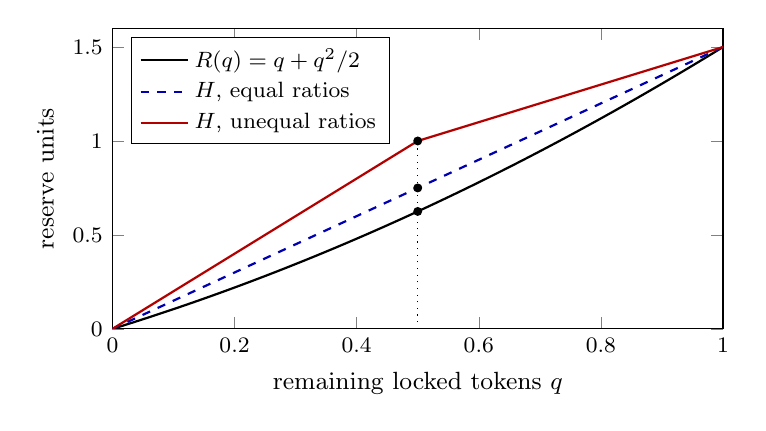
\begin{tikzpicture}
\begin{axis}[width=0.77\textwidth,height=5.4cm,
  xlabel={remaining locked tokens $q$},ylabel={reserve units},
  xmin=0,xmax=1,ymin=0,ymax=1.6,
  legend pos=north west,legend cell align=left,
  tick label style={font=\footnotesize},label style={font=\small},
  legend style={font=\footnotesize}]
\addplot[thick,black,domain=0:1,samples=101] {x+x*x/2};
\addlegendentry{$R(q)=q+q^2/2$}
\addplot[thick,dashed,blue!70!black,domain=0:1,samples=2] {1.5*x};
\addlegendentry{$H$, equal ratios}
\addplot[thick,red!70!black] coordinates {(0,0) (0.5,1) (1,1.5)};
\addlegendentry{$H$, unequal ratios}
\draw[thin,dotted] (axis cs:0.5,0) -- (axis cs:0.5,1);
\addplot[only marks,mark=*,mark size=1.4pt,black]
  coordinates {(0.5,0.625) (0.5,0.75) (0.5,1)};
\end{axis}
\end{tikzpicture}
\caption{The required reserve is the greatest vertical distance from $R$ to the debt envelope $H$. Both books have $L=1$ and $D=3/2$. Their maximum gaps occur at $q=1/2$ and are $1/8$ for equal ratios and $3/8$ for the two unequal ratios. These quantities are checked in script block CF01.}\label{cr:figure}
\end{figure}

For the linear price $p(q)=P+kq$, with $P>0$ and $k>0$, minimizing \eqref{cr:dmax} gives
\begin{equation}\label{cr:linearcapacity}
\frac{D_{\max}}L=
\begin{cases}
P, & W=0,\\[2pt]
P+\sqrt{2kW}, & 0<W\le kL^2/2,\\[2pt]
P+kL/2+W/L, & W>kL^2/2.
\end{cases}
\end{equation}
The interior minimizing depth is $\sqrt{2W/k}$. The formula describes cash coverage, not a positive residual for every borrower. An above-floor proportional loan can become worth less than its debt after a partial repayment, even when the committed reserve makes every free redemption payable. For example, in the one-token case above, $W=1/8$ pays the released half, but the remaining debt $3/4$ exceeds $R(1/2)=5/8$. A collateral-funded close is a separate requirement.


\section{The Reserve as an Extractable Subsidy}\label{sec:subsidy}

The reserve of \cref{cr:buffer} makes above-floor loans payable. It does not make them worth repaying. For exit routing, a holder whose tokens would redeem for a gross value $v$ per token receives $(1-f_s)v$ by redeeming and $(1-\phi)a$ by borrowing at the ratio $a$ and never repaying. Abandonment pays whenever $(1-\phi)\,a>(1-f_s)\,v$, the condition under which the floor-cap contract invites abandonment, with $\gamma\Pf$ replaced by $a$ \citep{extended}. For a holder who redeems at the floor, $v=\Pf$, and a ratio $a>\Pf$ satisfies the condition unless the fees are at least as large as the lending premium, $(1-f_s)/(1-\phi)\ge a/\Pf$. Under the floor cap, $a\le\gbar\Pf$, and a cap with $\gbar+\fsbar<1$ gives the opposite inequality at every sell fee within $\fsbar$; lending above the floor removes that guarantee.

Borrowers can do better than choose between repaying in full and abandoning. They can repay in part, redeem the collateral that the repayment releases, and abandon the rest. The next result says exactly how much this takes out.

\begin{proposition}[What a committed reserve can lose]\label{cr:extraction}
In the setting of \cref{cr:rights}, with no fees, let the book be safe under its repayment rights, that is, $W\ge W_{\min}$. Let a coalition hold all $L=S$ tokens, locked against the loans of the book, and let the reserve $W$ have been paid in by someone else.
\begin{enumerate}[label=(\alph*)]
\item If the coalition repays down to an attainable residual configuration with total lock $Q$ and total debt $B$, redeems the released tokens and never repays the rest, it receives $B-R(Q)$ more than by repaying every loan and redeeming every token. The supremum of this gain over attainable configurations, which is the maximum over their closure, is $W_{\min}$, the least reserve that \cref{cr:kernel} requires. Under proportional release the supremum is attained.
\item After a path that attains this maximum the issuer holds cash $W-W_{\min}$.
\item Under proportional release, a book that is admitted with total debt $D_{\max}$ of \eqref{cr:dmax} and $W>0$ has $W_{\min}=W$: the coalition can take the whole reserve.
\item For a coalition that buys the $L$ tokens from an empty curve and pays a buy fee $f_b$, an origination fee $\phi$ and a sell fee $f_s$, all proportional and paid out of the mechanism, the profit of the path in (a) is
\[
\Pi=B-R(Q)-f_b\,R(L)-\phi\,D-f_s\,\bigl[R(L)-R(Q)\bigr].
\]
\item Under the curve-valued contract of \cref{cr:nonlinear} every attainable configuration has $B\le R(Q)$, so the gain in (a) is never positive.
\end{enumerate}
\end{proposition}
\begin{proof}
Because the book is safe under its repayment rights, every repayment and redemption below can be executed; without that hypothesis $B-R(Q)$ is still the difference of the two cash flows as written, but the issuer may run out of cash before the redemption is paid. (a) Repaying down to the configuration costs $D-B$ and the released $L-Q$ tokens redeem for $R(L)-R(Q)$; repaying everything costs $D$ and returns $R(L)$. The difference is $B-R(Q)$. By \cref{cr:kernel} the least admissible reserve is the supremum of $\sum_ib_i-R(\sum_iq_i)$ over attainable configurations, equivalently its maximum over their closure, and it is at least zero because $(0,0)$ is attainable for every loan. (b) The proof of \cref{cr:kernel} gives the cash after the path as $W+R(Q)-B$. (c) Because $W>0$, the function $(R(q)+W)/q$ tends to infinity as $q\downarrow0$ and is continuous on $(0,L]$, so the infimum in \eqref{cr:dmax} is attained at some $q^\ast>0$, where $(D_{\max}/L)\,q^\ast=R(q^\ast)+W$. By concavity $H(q^\ast)\ge D_{\max}q^\ast/L$, so $H(q^\ast)-R(q^\ast)\ge W$, and admission requires $W_{\min}\le W$. (d) The purchase costs $(1+f_b)R(L)$, the loans pay out $(1-\phi)D$, the repayment costs $D-B$ and the redemption returns $(1-f_s)[R(L)-R(Q)]$; the sum is $\Pi$. (e) The persistent condition \eqref{cr:nonlinearcover} holds at every attainable configuration, so $B\le\gbar\sum_iR(q_i)\le R(Q)$ by \eqref{cr:superadd}.
\end{proof}

The reserve that makes a proportional book safe is thus exactly the amount that a coalition of its borrowers can extract from it. Take $R(q)=q+q^2/2$, $L=S=1$ and $W=0.08$, which is below the threshold $kL^2/8=0.125$ at which $D_{\max}$ passes the redemption value $R(L)$ of the whole collateral. Then $D_{\max}=1.4<R(1)=1.5$, so repaying in full is still better than abandoning in full. But buying the token for $1.5$, borrowing $1.4$, repaying $0.84$ to release $0.6$ tokens, redeeming them for $1.02$ and leaving $0.4$ tokens locked against a debt of $0.56$ nets $0.08$: the whole reserve. The issuer is left with no cash and a residual loan of $0.56$ against collateral that redeems for $R(0.4)=0.48$: the loan is under-collateralized, in a state that remains safe under its repayment rights. With all three fees at $1\%$ the profit is $0.0408$ (script block N16). The statement is about a strategy that is available, under the stated assumptions on access and on who funded the reserve; it is not a prediction of what borrowers do, and a borrower who paid in the reserve counts that payment as a cost. The borrower's position is the residual claim of the corporate-debt model, the right to recover the collateral by paying the debt or to walk away \citep{merton1974}, and $W_{\min}$ is capital held against the worst admissible scenario, in the spirit of, though not shown to satisfy the axioms of, a coherent risk measure \citep{artzner1999}.

Two consequences follow. At the maximum admitted credit \eqref{cr:dmax}, the committed reserve is exposed to complete loss under the strategy above: it is first-loss capital for that path, though other repayment paths return it. And the amount that must stay committed is the current $W_{\min}$, not $W$: a repayment narrows the set of residual configurations and can lower the requirement, after which the difference may be withdrawn while the loan is open. In the example, repaying $1.12$ leaves $0.2$ tokens against a debt of $0.28$ and a requirement of $0.06$, so $0.02$ of the reserve is free. A path that repays and abandons can instead use up the cash and leave the remaining requirement committed for good. The curve-valued contract of the next section does not have the defect, by part~(e), and under $\gbar+\fsbar<1$ redeeming a lock pays more than abandoning it.


\section{More Credit with a Different Release Rule}\label{cr:nonlinear}


There is also a way to use the curve premium without an additional committed reserve. Suppose a partial repayment reduces debt but releases no collateral until the loan is fully repaid. By \cref{cr:kernel}, with $W=0$ such a book is safe under all repayments if and only if
\begin{equation}\label{cr:fullrelease}
d_i\le R(\ell_i)\qquad\text{for every loan}.
\end{equation}
Each remaining debt is at most its initial debt at the unchanged lock, and fully repaid loans disappear. Thus \eqref{cr:fullrelease} is the largest per-loan cap compatible with these rights and with the possibility that every other borrower exits.

Partial collateral release is possible if its amount is changed. Consider the operations of \cref{sec:model}, with the following replacements. The persistent loan condition is
\begin{equation}\label{cr:nonlinearcover}
d_i\le\gbar R(\ell_i),\qquad 0<\gbar\le1.
\end{equation}
A borrow is guarded by $d_i+b\le\gamma R(\ell_i+\ell^+)$, with $0<\gamma\le\gbar$. A partial repayment of $r$ may release $u\in[0,\ell_i]$ only if $d_i-r\le\gbar R(\ell_i-u)$; full repayment releases the whole lock. A reshape preserves \eqref{cr:nonlinearcover} for every loan under the new $R$, as well as satisfying (G1) and (G2). Custody, the definitions of $A,D,W$, and the remaining operations are unchanged. The release rule and the debt anchor are both different from those of the original model.

\begin{proposition}[Safety with a curve-valued lock]\label{cr:nonlinearsafety}
These operations preserve custody, \eqref{cr:nonlinearcover} and $A+D\ge R(S)$. Every free-token gross redemption and every admitted loan can be paid in full, without any repayment by another borrower. If proportional sell fees satisfy $f_s\le\fsbar$ and $\gbar+\fsbar\le1$, every loan can also be closed from its own collateral. The close leaves a positive residual when $\gbar+\fsbar<1$.
\end{proposition}
\begin{proof}
By \eqref{cr:superadd}, $D\le\gbar\sum_iR(\ell_i)\le\gbar R(L)$. This is the aggregate bound used in the coverage and cash-payout steps of \cref{thm:safety}. The modified borrow, repayment and reshape guards preserve the new individual condition; the other induction steps are unchanged. In particular a borrow gives $D+b\le\gbar R(S)$, so $A-b\ge(1-\gbar)R(S)$. For a close, monotonicity of $p$ gives
\[
R(S)-R(S-\ell_i)\ge R(\ell_i),
\]
and net proceeds are therefore at least $(1-\fsbar)R(\ell_i)\ge d_i$. Let the borrower close and redeem in one operation, in which the debt is netted against the proceeds of the lock. If $G=R(S)-R(S-\ell_i)$ is the gross return, the combined reserve outflow is at most $G-d_i$, and
\[
A-(G-d_i)=W+R(S-\ell_i)-(D-d_i)\ge0,
\]
because the other locks total at most $S-\ell_i$ and satisfy \eqref{cr:superadd}. With a strict inequality between the caps, the borrower's residual is at least $(1-\fsbar-\gbar)R(\ell_i)>0$.
\end{proof}

Since $R$ is strictly increasing, the largest release allowed by the new repayment guard is
\begin{equation}\label{cr:maxrelease}
u_{\max}(r)=\ell_i-R^{-1}\!\left(\frac{d_i-r}{\gbar}\right).
\end{equation}
At a loan's limit $d_i=\gbar R(\ell_i)$, convexity implies $u_{\max}(r)\le\ell_i r/d_i$. Paying half the debt therefore need not release half the tokens. For the unit lock of \cref{cr:rights} with $R(q)=q+q^2/2$, debt $3/2$ and $\gbar=1$, repaying $3/4$ releases $2-\sqrt{5/2}\simeq0.418861$ tokens, whose curve return is exactly $3/4$. An integer implementation must round the remaining required lock upward; this section's result is real-valued, not a verification of such an implementation.

\paragraph{The stronger reshape guard matters.}
Let $p(q)=1+q$, $S=2$, one token locked against $d=3/2$, one token free, and $A=5/2$. Replace the curve by prices $1$ on $[0,1)$ and $3$ on $[1,2)$. The floor remains $1$ and total reserve remains $R(2)=4$, so (G1) and (G2) hold. But the new $R(1)=1$ no longer covers the loan, and the free token's return $3$ exceeds cash. Requiring $d_i\le\gbar R_{p'}(\ell_i)$ rejects this change. A sufficient condition that avoids inspecting each loan is $R_{p'}(z)\ge R_p(z)$ for all $z\le S$, together with funding; a floor raise that lifts every price below a level $y$ to $y$ and leaves the others unchanged satisfies this condition. The new release rule can depend on the curve, so results that assume a release rule depending only on the loan, such as the deferral result of the extended version, do not automatically extend to it.

\subsection{Pooling, splitting and independent exit}\label{cr:pooling}

The additional capacity in \eqref{cr:fullrelease} depends on position size. Combining locks $x,y$ increases the maximum debt by
\begin{equation}\label{cr:poolgain}
R(x+y)-R(x)-R(y)
=\int_0^y[p(x+u)-p(u)]\,du\ge0.
\end{equation}
For $p(q)=P+kq$ the gain is $kxy$. This is the value, in lending capacity, of keeping the collateral subject to a joint release condition. A split need not be feasible after the additional credit has been drawn.

\begin{proposition}[Arbitrary independent splitting]\label{cr:splitting}
Suppose $W=0$ and a loan $(\ell,d)$ may be split into $n$ independently repayable loans $(\ell/n,d/n)$ for every positive integer $n$. If the resulting book must remain safe when any subset of the other loans is fully repaid and its released tokens are redeemed, then $d\le\Pf\ell$.
\end{proposition}
\begin{proof}
Leave one of the $n$ loans outstanding and repay all others. \Cref{cr:kernel} requires $d/n\le R(\ell/n)$. Hence $d/\ell\le R(\ell/n)/(\ell/n)$ for every $n$, whose limit is $\Pf$.
\end{proof}

There is consequently no gain from the curve premium while retaining all three properties: no committed reserve, arbitrary proportional splitting, and independent repayment and exit. A pool can obtain more credit only by changing one of those properties. Nor is the gain universal across borrowers: on a stepped curve, $R(\ell)=\Pf\ell$ for $\ell\le S_0$, so small positions entirely within the floor capacity obtain no extra credit from \eqref{cr:fullrelease}.


\section{Algorithms and Executable Checks}\label{sec:algo}

\subsection{Constructing the proportional envelope}\label{cr:algorithm}

Order the loans so that $a_1\ge\cdots\ge a_n$, where $a_i=d_i/\ell_i$. Write $Q_j=\sum_{i\le j}\ell_i$, $B_j=\sum_{i\le j}d_i$, and $Q_0=B_0=0$. For $Q_{j-1}\le q\le Q_j$,
\begin{equation}\label{cr:piecewiseH}
H(q)=B_{j-1}+a_j(q-Q_{j-1}).
\end{equation}
To prove the formula, if an allocation retains some collateral from a smaller-ratio loan while a larger-ratio loan is not fully retained, transfer the smaller of the available two amounts to the larger-ratio loan. Total collateral stays fixed and remaining debt does not decrease. Repeating this exchange gives \eqref{cr:piecewiseH}. Ties have no effect on $H$.

Suppose the input represents $p$ by $m$ intervals with rational endpoints, rational affine prices $p(q)=c_j+k_jq$ on each interval, $k_j\ge0$, and non-negative jumps between intervals. The reserve function is then continuous and piecewise quadratic, with exact rational values at rational arguments. Restrict all intervals to $[0,L]$ and merge their endpoints with the $Q_j$. On any interval of this merged partition,
\[
H(q)-R(q)=b+aq-cq-\tfrac12 kq^2
\]
for an appropriate constant $b$. A maximum on that interval is attained at an endpoint or, if $k>0$, at $q=(a-c)/k$ when that point lies in the interval. If $k=0$, endpoints suffice, including the case of a constant difference. Evaluating this finite candidate list therefore finds $W_{\min}$ exactly.

Sorting requires $O(n\log n)$ comparisons. With price intervals already ordered, the merged scan takes $O(n+m)$ arithmetic operations; the number of candidates is linear in $n+m$. Rational additions, products and comparisons have polynomial bit complexity in the input length. This establishes polynomial-time exact evaluation for this representation. It makes no such computational claim for an unspecified real-valued function $p$.

Concavity also gives a useful check: the slopes of $H-R$ cannot increase. A maximizer lies where these slopes change from non-negative to non-positive, or at an endpoint. The candidate method used in the script checks every merged interval, rather than relying on an approximate numerical root. The equal-ratio comparison in \cref{cr:capacity} needs no uniqueness of this maximizer. The closed form \eqref{cr:linearcapacity} follows by minimizing $P+kq/2+W/q$: for $W>0$ its unconstrained minimum is at $q=\sqrt{2W/k}$; if that depth exceeds $L$, the constrained minimum is at $L$. For $W=0$ the infimum is the limit $P$ at zero.

\subsection{Guards for a proportional book}\label{cr:guards}

Let the extended invariant be custody, the amount-domain conditions, and $W\ge W_{\min}$, with proportional release. This implies the immediate coverage condition because $H(L)=D$:
\[
A=R(S)-D+W\ge R(S)-R(L)\ge0.
\]
After a repayment, each surviving loan has the same ratio $a_i$ and a smaller collateral capacity. Its remaining residual configurations form a subset of the earlier ones, so the maximum defining $W_{\min}$ cannot increase. The repayment leaves $W$ unchanged. A gross sale leaves both the loan book and $W$ unchanged. A sale with a smaller total reserve outflow increases $W$. A purchase whose reserve inflow covers its curve cost also increases $W$ and leaves the existing loan book unchanged.

A withdrawal of $w$ changes only $W$ and cash, so its exact safety guard is $w\le W-W_{\min}$. This bound implies that the withdrawal is affordable: $W_{\min}\ge D-R(L)$ and $R(L)\le R(S)$ give
\[
W-W_{\min}\le W-D+R(L)\le A.
\]
For a proposed new loan or top-up, calculate the resulting debt and locks and the total cash outflow. Accept only if the resulting $W'$ satisfies $W'\ge W_{\min}'$. This implies non-negative resulting cash by the preceding immediate-coverage argument. If the outflow is the gross new debt, then $W'=W$; a retained origination fee increases it. The use of resulting quantities is essential: checking only the old envelope is insufficient.

For a reshape with external inflow $c$, the proposed surplus is $W'=A+c+D-R_{p'}(S)$. Require $W'\ge W_{\min}(p',\{\ell_i,d_i\})$. Proportional rights do not change with the schedule, so this is precisely the condition for the continuation with the new curve. A floor-monotonicity rule can additionally protect the promised floor; it is not a substitute for the new buffer test. For a more general release contract, the test must use its actual residual-pair sets, not the proportional envelope. Nothing here authorizes changing a borrower's contractual release rights merely to make a proposed reshape pass.

\subsection{Whole-position release}\label{sec:whole}

If a lock can only be released in full, the configurations to test are the subsets of loans, and the least reserve $W^{\mathrm{whole}}$ is the largest value of $\sum_{i\in J}d_i-R(\sum_{i\in J}\ell_i)$ over subsets $J$. Computing it exactly is hard in general: deciding safety is coNP-complete already for $R(q)=q+q^2/2$, by a reduction from PARTITION, although for integer locks of total $L$ a pseudopolynomial dynamic program decides it with $O(nL)$ rational arithmetic operations (\cref{cr:complexity}). A design does not need the exact value. The sorted envelope is a safe guard for whole-position release too, and it over-reserves by at most the largest amount by which a single loan exceeds the floor value of its lock:
\[
W^{\mathrm{whole}}\;\le\;W^{\mathrm{prop}}\;\le\;W^{\mathrm{whole}}+\max_i\,(d_i-\Pf\ell_i)^+ .
\]
The constant is sharp in general and improves to $\tfrac14$ for linear prices (\cref{cr:guardbound,cr:guardsharp}).

\subsection{What is checked, and how}\label{sec:evidence}

Three kinds of evidence support different parts of the paper, and we keep them apart.

\emph{Machine-checked.} \Cref{thm:safety} is formalized in Lean~4 with Mathlib (\texttt{lean/Safety.lean}): the invariant, the step relation with every operation of \cref{sec:model}, preservation, and payability of sales, loans and skims on every reachable path. The formal statements are in \cref{app:lean}. The formalization covers the real-valued floor-cap contract. It does not cover the results of \cref{sec:credit,sec:subsidy,cr:nonlinear}.

\emph{Implemented and tested.} A Solidity implementation of the floor-cap contract and an integer reference model in Python accompany the paper. The contract agrees with the model on every one of 30{,}000 replayed operations, including 1{,}441 attempted replacements of the schedule, of which 1{,}048 are admissible and 393 must be refused; stateful tests check the invariant after random sequences of calls, and the floor invariant is shown to fail when the floor guard is deleted from the contract; 189 tests pass in all. The contract is tested, not verified, and it implements neither of the two extensions.

\emph{Proved on paper and checked in exact arithmetic.} The results of \cref{sec:credit,sec:subsidy,cr:nonlinear} are proved in the text. A script in exact rational arithmetic recomputes the examples of \cref{sec:credit,cr:nonlinear}, compares the sorted-envelope algorithm with exhaustive enumeration of residual states on 240 books (160{,}640 states, no mismatch), follows 144 repayment paths and 328 closes of the curve-valued contract without a shortfall, enumerates 2{,}696 subsets against the dynamic program, and confirms that four deliberately unsafe variants (coverage of the current state only; an average-ratio proxy for the reserve; a skim of the committed reserve; the old reshape guards with the new loan cap) each admit a path with a cash shortfall. These are finite checks of the calculations; the general statements rest on the proofs. The remaining numerical examples are evaluated by a second script, in floating point where a square root occurs.

\section{Design Consequences and Limits}\label{sec:consequences}

\subsection{The three contracts compared}\label{cr:compare}


\Cref{tab:contracts} puts the floor-cap contract beside the two extensions, with numbers for the linear price $p(q)=1+q$, a total lock of one token, loan caps of one and no fees (script block N17). The buffered contract adds $40\%$ to the credit of every lock for a reserve of $0.08$, and exposes that reserve in full. The curve-valued contract needs no reserve and has no such exposure, but what it adds depends on the size of a lock: half the lock size in relative terms on this curve, so $5\%$ for a lock of $0.1$ and $50\%$ for a single lock of the whole supply, and nothing at all for a lock that fits inside a flat floor segment. Ten equal locks together obtain $5\%$, one pooled lock $50\%$; the difference is the price of independent exit. Whether either extension is worth its cost depends on the distribution of lock sizes and on what the reserve could otherwise earn, which we do not measure.

\begin{table}[t]
\centering\small
\caption{The floor-cap contract and the two extensions of this section. Numbers are for $p(q)=1+q$, total lock $L=1$ (floor value $1$), caps $\gamma=\gbar=1$ and no fees; ``gain'' is the coalition gain of \cref{cr:extraction}.}\label{tab:contracts}
\begin{tabularx}{\textwidth}{@{}>{\raggedright\arraybackslash}p{0.2\textwidth}>{\raggedright\arraybackslash}X>{\raggedright\arraybackslash}X>{\raggedright\arraybackslash}X@{}}
\toprule
 & Floor cap (\cref{sec:model}) & Committed reserve, proportional release & Curve-valued lock\\
\midrule
Credit of a lock $\ell$ & $\Pf\ell=\ell$ & $(D_{\max}/L)\,\ell=1.4\,\ell$ at $W=0.08$ & $R(\ell)=\ell+\ell^2/2$\\
Aggregate credit & $1$ & $1.4$ & $1.05$ (ten locks) to $1.5$ (one lock)\\
Committed capital & none & $W=0.08$ & none\\
Largest gain & $0$ & $W_{\min}=0.08$, the whole reserve & $0$\\
Release on partial repayment & proportional & proportional & less than proportional at the limit: $0.419$ of a unit lock for half the debt\\
Splitting a position into independent loans & leaves credit unchanged & leaves credit unchanged & reduces capacity; unrestricted proportional splitting forces the floor bound (\cref{cr:splitting})\\
Guards on curve changes & (G1), (G2) & reserve test with the new curve & (G1), (G2) and the loan condition under the new curve\\
Check at a borrow & one inequality per loan & sorted envelope of the whole book & one inequality per loan, with $R$\\
Evidence in this paper & Lean proof, reference model, contract, tests & proofs, exact finite checks & proofs, exact finite checks\\
\bottomrule
\end{tabularx}
\end{table}

\subsection{Who funds the reserve}

\Cref{cr:extraction} changes how a committed reserve should be read. It protects those who redeem. Under proportional release it is also what a coalition holding all the tokens \emph{can} take: with no fees and a reserve funded by others, at most $W_{\min}$, and all of $W$ at the maximum admitted credit. With fees, the gain is reduced by the amounts in part~(d) of the proposition and can be negative. We have proved that the strategy is available and what it pays at most; we have not valued the option that it gives borrowers, and we do not predict that it is exercised. A sponsor who funds a reserve to offer more credit should nevertheless count it as capital exposed to that strategy and not as idle liquidity. If the coalition funds the reserve itself, the contribution has to be subtracted from its proceeds, and under the same assumptions its net gain is at most $W_{\min}-W\le0$; the reserve still does its work of covering redemptions, and it can still move value between borrowers who contribute and repay unequally. The curve-valued contract avoids the exposure by never lending more than the reserve value of what stays locked, and pays for that with the restrictions of \cref{cr:pooling}.

\subsection{What safety does not give}

The results above are statements about a balance sheet in units of the reserve asset. They do not show that anyone wants the credit. The extended version \citep{extended} analyzes the floor-cap contract further and finds that safety and viability separate there too. For a price-taking borrower who values cash flows, holds tokens that pay nothing and has no use for them in the meantime, deferring the repayment of a loan without carrying cost is weakly optimal. And in a stationary equilibrium at the floor, with given arrivals and no retained surplus, entrants as a group pay for the reserve that a rising floor needs and for the time their capital spends in the system: the token-weighted mean value of entering is negative whenever the floor grows more slowly than holders discount and the loan cap is below the net floor. In event data from one deployed system of this kind, $\ELeverAmtPct\%$ of new debt by amount finances purchases of more of the same token. A theory of that leveraged demand is the missing piece, and neither version of this paper supplies it.

Four further limits apply. The floor never falls in units of the reserve asset, which says nothing about the value of that asset. The capacity results fix the curve; a design that changes the curve needs the guards of \cref{cr:guards} or the stronger reshape guard of \cref{cr:nonlinear}. The alternative contracts are specified and proved on paper, and are neither implemented nor machine-checked. And we have not measured how much credit the curve-valued contract would add at the lock sizes of a real system; for a lock that fits inside a flat floor segment it adds nothing.

\paragraph{Disclosure.} The author is a co-founder of House Markets, which develops token issuance and credit mechanisms of the kind analyzed here, and is a co-author of \vone, on which the floor-cap contract builds. The author holds no tokens of Baseline or Nirvana.

\section{Conclusion}

Lending the redemption reserve against locked tokens is safe today whenever debt is covered by the reserve of the locked part of the curve. It stays safe only if residual debt is covered by the committed reserve plus the reserve of the residual lock in every state that borrowers can reach by repaying, and this is a condition on the withdrawal rights that the loans carry. With proportional release and no committed reserve, the condition is the floor cap, loan by loan. Lending more needs a reserve whose exact size is the largest gap between a sorted debt envelope and the reserve curve, and with no fees that same number is the most that a coalition holding all the tokens can take out of a reserve funded by others. A contract that releases collateral along the curve lends more without a reserve and without that exposure, and gives up proportional release, free splitting and the simple reshape guards. More credit therefore has a price in capital or in withdrawal rights, and the choice between the two is a design decision that the accounting makes explicit.


\bibliographystyle{plainnat}
\bibliography{references}

\appendix

\section{Formal Statements}\label{app:lean}

The file \texttt{lean/Safety.lean} states the following, in the namespace \texttt{FloorCredit}. We give each statement in the notation of the paper, with the name it has in the file.

\begin{description}[leftmargin=1.2em,itemsep=3pt]
\item[\texttt{Sched R Pf C}] (hypothesis on the reserve function). $\Pf>0$, $C>0$, $R(0)=0$, and $R(b)-R(a)\ge\Pf\,(b-a)$ for all $0\le a\le b\le C$. Nothing else is assumed about $R$; in particular $p$ need not be monotone.
\item[\texttt{State}, \texttt{Valid}, \texttt{Inv}.] A state is $(R,\Pf,C,S,A,\gamma,h,\ell,d)$ with $h,\ell,d$ indexed by a finite set of accounts. \texttt{Valid} is: \texttt{Sched}; $0\le S\le C$; $A\ge0$; $0<\gamma\le\gbar$; $h_u,\ell_i,d_i\ge0$. \texttt{Inv} is \texttt{Valid} together with (J1) $\sum_uh_u+\sum_i\ell_i=S$, (J2) $d_i\le\gbar\Pf\ell_i$ for every $i$, and (J3) $R(S)\le A+\sum_id_i$.
\item[\texttt{Step}.] The relation between a state and its successor under one operation whose guard holds: buy, sell, borrow, full repayment, partial repayment with any release $u\ge0$ such that $u\,d_i\le\ell_i\,r$, transfer of free tokens between two distinct accounts, change of $\gamma$, reshape with (G1) and (G2), skim, and capped accrual of debt, an operation of the extended version.
\item[\texttt{coverage}.] If \texttt{Inv} holds, $\gbar\ge0$ and $0\le x\le S-L$, then $R(S)-R(S-x)+(1-\gbar)R(L)\le A$.
\item[\texttt{sell\_payable}, \texttt{borrow\_payable}, \texttt{skim\_payable}.] If \texttt{Inv} holds and $0\le\gbar\le1$: a holder's sale of $0<x\le h_u$ satisfies $R(S)-R(S-x)\le A$; a loan $b$ whose guard holds satisfies $b\le A-(1-\gbar)R(S)$; a skim whose guard holds satisfies $w\le A$.
\item[\texttt{inv\_empty}.] The empty state with a \texttt{Sched} reserve function and $0<\gamma\le\gbar$ satisfies \texttt{Inv}.
\item[\texttt{step\_preserves}.] If $0<\gbar\le1$, \texttt{Inv} holds in $s$ and \texttt{Step} relates $s$ to $s'$, then \texttt{Inv} holds in $s'$.
\item[\texttt{reach\_inv}, \texttt{reach\_sell\_payable}.] If $0<\gbar\le1$ and \texttt{Inv} holds in $s_0$, then \texttt{Inv} holds in every state reachable from $s_0$ by finitely many steps, and in every such state every sale of free tokens satisfies $R(S)-R(S-x)\le A$.
\item[\texttt{sched\_of\_integral}.] If $C>0$, $p$ is non-decreasing on $[0,C]$ and $p\ge\Pf>0$ there, then $R(x)=\int_0^xp$ satisfies \texttt{Sched}.
\end{description}

From the directory \texttt{lean/}, \texttt{lake build} checks the file with the pinned toolchain and Mathlib revision. Our run used \texttt{lake env lean Safety.lean} in a project with the same toolchain and the same Mathlib revision; it ends without output, and \texttt{\#print axioms} reports \texttt{propext}, \texttt{Classical.choice} and \texttt{Quot.sound} for the last three theorems.

\section{Whole-Position Release: Complexity and the Envelope Guard}\label{cr:complexity}

With whole-position release, full repayment releases the entire lock; a partial repayment, if allowed, releases none. For testing the greatest cash requirement it suffices to consider loans that are either unchanged or fully repaid. A partial repayment reduces debt at an unchanged lock and cannot increase the shortfall. Thus \cref{cr:allpairs} becomes the finite family
\begin{equation}\label{cr:subsets}
\sum_{i\in J}d_i\le W+R\!\left(\sum_{i\in J}\ell_i\right)
\qquad\text{for every subset }J.
\end{equation}
For $W=0$ this reduces to the per-loan conditions $d_i\le R(\ell_i)$ by \eqref{cr:superadd}. With a shared positive reserve, testing all subsets can instead be a combinatorial problem.

\begin{samepage}
\begin{proposition}[Complexity of whole-position coverage]\label{cr:hardness}
Consider the decision problem \eqref{cr:subsets} with positive integer collateral amounts encoded in binary, positive rational debts, non-negative rational $W$, and $R(q)=q+q^2/2$ on a bounded domain containing the supply. Deciding whether the book is safe is coNP-complete. With integer locks of total $L$, a dynamic program with $O(nL)$ rational arithmetic operations decides it. Thus the hardness established here is weak; there is no claim of strong hardness or intractability for every class of curves and books.
\end{proposition}
\end{samepage}
\begin{proof}
An unsafe subset is a polynomial-size certificate: sum its integer locks and rational debts and compare them with $W+R(q)$ using exact rational arithmetic. The complement of safety is therefore in NP.

Reduce from PARTITION, whose input is a list of positive integers $w_i$ summing to $2B$, and whose question is whether a subset sums to $B$ \citep{karp1972}. The even-total restriction does not change NP-completeness, since odd-total instances are immediate no instances. Set
\[
\ell_i=w_i,\qquad d_i=(1+B)w_i,\qquad
W=\frac{B^2}{2}-\frac14,\qquad S=L=2B.
\]
All numbers have polynomial encoding length. A schedule $p(q)=1+q$ on $[0,2B+1)$ meets \cref{def:schedule}. For a retained subset of total lock $x$, the debt minus curve reserve is
\begin{equation}\label{cr:partitiondeficit}
(1+B)x-R(x)=Bx-\frac{x^2}{2}
=\frac{B^2}{2}-\frac{(x-B)^2}{2}.
\end{equation}
If $x=B$, it exceeds $W$ by $1/4$. Otherwise $x$ is an integer with $|x-B|\ge1$, so it is at most $B^2/2-1/2<W$. There is an unsafe subset exactly when the PARTITION instance is a yes instance. Hence unsafety is NP-hard and safety is coNP-hard; membership proves completeness.

For the dynamic program, let $M_j(x)$ be the largest debt of a subset of the first $j$ loans with total lock exactly $x$, or $-\infty$ if none exists. Start with $M_0(0)=0$ and all other values $-\infty$, and use
\[
M_j(x)=\max\{M_{j-1}(x),\ M_{j-1}(x-\ell_j)+d_j\},
\]
omitting the second term for $x<\ell_j$. Test $M_n(x)\le W+R(x)$ for all $0\le x\le L$. There are $O(nL)$ states, and sums and comparisons of the rational debts have polynomial bit length. This is a pseudopolynomial algorithm because the binary encoding of $L$ can be much shorter than $L$.
\end{proof}

\paragraph{Reachability of the constructed book.}
The reduction does not rely on a negative initial cash balance. It has $D=(1+B)2B=R(2B)$ and $A=W\ge0$. It can also be reached without violating instantaneous gross coverage in a model that replaces the floor loan cap by the immediate aggregate test. Buy all $2B$ tokens at curve cost, contribute $W$, and originate every lock $w_i$ with debt $w_i$. At this stage all tokens are locked and debt is $2B$. Top up each debt to $(1+B)w_i$. Total debt never exceeds $R(2B)$, cash never falls below $W$, and there are no free tokens during the top-ups. If a partition exists, fully repay the complementary loans and redeem their $B$ released tokens. The cash shortfall is $1/4$. These top-ups are deliberately outside the original floor cap; the construction is not a counterexample to \cref{thm:safety}.

The complexity comparison also has a limited meaning. Whole-position release admits fewer repayment paths than proportional release, so for the same initial book its minimum required reserve is no greater. Its subset condition can nevertheless be harder to evaluate exactly. The one-dimensional envelope solves the divisible problem because every fractional residual allocation is permitted; it is not the exact envelope for a discrete book.

\begin{proposition}[The envelope as a guard for whole-position release]\label{cr:guardbound}
For the same book and curve let $W^{\mathrm{prop}}$ be the reserve \eqref{cr:wmin} required under proportional release and $W^{\mathrm{whole}}$ the least $W$ satisfying \eqref{cr:subsets}. Then
\[
W^{\mathrm{whole}}\;\le\;W^{\mathrm{prop}}\;\le\;W^{\mathrm{whole}}+\max_i\,(d_i-\Pf\ell_i)^+ .
\]
\end{proposition}
\begin{proof}
Every whole-position configuration is a proportional one, which gives the first inequality. For the second, let $q^\ast$ maximize $H-R$ and let $j$ be the index with $Q_{j-1}\le q^\ast\le Q_j$ in the order of \cref{cr:algorithm}, so that $H(q^\ast)=B_{j-1}+\theta d_j$ and $q^\ast=Q_{j-1}+\theta\ell_j$ with $0\le\theta\le1$. The subset of the first $j-1$ loans gives $W^{\mathrm{whole}}\ge B_{j-1}-R(Q_{j-1})$. Hence
\[
W^{\mathrm{prop}}-W^{\mathrm{whole}}\le\theta d_j-\bigl[R(Q_{j-1}+\theta\ell_j)-R(Q_{j-1})\bigr]\le\theta\,(d_j-\Pf\ell_j)
\]
by \cref{lem:R}, and the right side is at most $(d_j-\Pf\ell_j)^+$.
\end{proof}

A contract with whole-position release can therefore use the sorted envelope as its guard. For a curve given by $m$ price intervals as in \cref{cr:algorithm}, the guard takes $O(n\log n+m)$ comparisons and arithmetic operations (bit complexity aside), it is safe, and it asks for more reserve than necessary by at most the largest amount by which a single loan exceeds the floor value of its lock; for an empty book that maximum is zero. The hardness result above concerns the exact requirement and is no obstacle to a design. The dynamic program can be impractical when the total collateral remains large after dividing the locks by their greatest common unit, since its table has one row per unit; the envelope guard does not depend on the magnitude of the collateral.

The constant $1$ in the bound cannot be improved in general, and it can be improved for linear prices.

\begin{corollary}[Sharpness]\label{cr:guardsharp}
(a) For every $\varepsilon\in(0,1)$ there is a schedule and a single loan with $W^{\mathrm{whole}}=0$, $(d-\Pf\ell)^+=1$ and $W^{\mathrm{prop}}=1-\varepsilon$. (b) For a linear price $p(q)=\Pf+kq$ with $k\ge0$,
\[
W^{\mathrm{prop}}-W^{\mathrm{whole}}\;\le\;\tfrac14\,\max_i\,(d_i-\Pf\ell_i)^+ ,
\]
and the factor $\tfrac14$ is attained.
\end{corollary}
\begin{proof}
(a) Let $p=1$ on $[0,1-\varepsilon)$ and $p=1+1/\varepsilon$ on $[1-\varepsilon,1)$, and take one loan with $\ell=1$, $d=2$. Then $R(1)=2=d$, so $W^{\mathrm{whole}}=0$, while $H(q)-R(q)=2q-q=q$ on $[0,1-\varepsilon]$ gives $W^{\mathrm{prop}}=1-\varepsilon$. (b) If $H-R$ is maximal at a point $Q_j$ of the partition, the gap is zero. Otherwise the maximum is at an interior point $q^\ast=Q_{j-1}+\theta\ell_j$ with $0<\theta<1$ and $k>0$, where the slope condition is $a_j=\Pf+kq^\ast$. On $[Q_{j-1},Q_j]$ the function $H-R$ is a quadratic with leading coefficient $-k/2$ and maximum at $q^\ast$, so it falls short of its maximum by $k(\theta\ell_j)^2/2$ at $Q_{j-1}$ and by $k((1-\theta)\ell_j)^2/2$ at $Q_j$. Both endpoints are whole-position configurations, so the gap is at most $\tfrac12k\ell_j^2\min\{\theta^2,(1-\theta)^2\}$. The slope condition gives $d_j-\Pf\ell_j=k\ell_jq^\ast\ge k\theta\ell_j^2$. The ratio of the two is at most $\min\{\theta^2,(1-\theta)^2\}/(2\theta)\le\tfrac14$, with equality only at $\theta=\tfrac12$ and $Q_{j-1}=0$. One loan with $\Pf=k=\ell=1$ and $d=R(1)=\tfrac32$ attains it: $W^{\mathrm{whole}}=0$, $W^{\mathrm{prop}}=\tfrac18$ and $d-\Pf\ell=\tfrac12$.
\end{proof}

Script block N15 of the supplementary material checks the inequalities of \cref{cr:guardbound,cr:guardsharp} on 3{,}000 random books with linear prices in exact arithmetic, and evaluates the example of part~(a).


\section{Reproduction}\label{app:repro}

The supplementary material contains the Lean file, the contract with its tests, the reference model, the scripts and their saved outputs. The Python scripts need Python~3 and no packages.
\begin{sloppypar}
\begin{itemize}
\item \texttt{python3 -I scripts/credit\_frontier.py} runs the exact-rational checks of \cref{sec:evidence}.
\item \texttt{python3 -I scripts/numbers.py} prints the numerical examples; blocks N14 to N17 concern this version.
\item \texttt{python3 -I scripts/test\_model.py 20000 300} runs the randomized tests of the reference model.
\item From \texttt{lean/}, \texttt{lake build} checks the formal proof. From \texttt{contracts/}, \texttt{forge test} runs the contract tests.
\end{itemize}
\end{sloppypar}

\end{document}
